
\section{Placement}
\label{sec:placement}
So far we have only dealt with the technology where we consider the problem space and adress the constraints of the hardware architecture. 
For every constraint, we devise a solution to fully address it or a simplification that sacrifices some optimization but reduces the complexity of the problem space. 

Now that we have dealt with the bulk of these constraints and squared them away into self-contained \texttt{SiteInst}s, we can now apply some general optimization algorithms to finally address our optimization objective, which is to place these \texttt{SiteInst} objects onto the device while minimizing wirelength. 

\subsection{Simulated Annealing}
\label{subsec:simulated_annealing}

In this paper we implement and present a basic Simulated Annealing (SA) placer. 
As mentioned in the Introduction, SA is a metaheuristic that approximates a global optimum in a large optimization search space. 
SA does not guarantee a globally optimal solution, but provides solutions that are often "good enough", especially when finding an approximate global optimum is more important than finding a precise local optimum in a fixed amount of time. 
SA is typically employed in discrete combinatorial optimization problems like the travelling salesman problem or job-shop scheduling. 
It is directly inspired by Annealing in metallurgy, which is the physical process of heating a metal above its crystallization temperature, allowing its atoms to migrate through the crystal lattice, and slowly cooling it to allow its atoms to recrystallize into a more desirable structure, such as one that minimizes structural defects 

The state \(s\) of the system and the function \(E(s)\) to be minimized is analogous to the internal energy of the system. 
In metallurgic Annealing, the state \(s\) represents the position of every atom in the metal object at any given snapshot in time, while \(E(s)\) represents the defectiveness in the metal's structure however that may be quantified. 
In the context of our SA placer, the state \(s\) represents the placement of every \texttt{SiteInst} on the \texttt{device} at any given iteration, while \(E(s)\) represents the total wirelength (HPWL) of \texttt{Net}s between all \texttt{SiteInst}s of the current placement.
The goal of SA is to bring the system from some initial state to a state with lower energy until some stopping criterion is met, whether that be when a computational budget is exceeded, an energy budget is met, or until the energy's rate of change approaches zero. 

At each step or iteration, the algorithm considers some neighboring state \(s^*\). 
If \(s^*\) has a lower energy than \(s\), then the state transition from \(s\) to \(s^*\) is accepted outright.
If \(s^*\) has a higher energy, then it can probabilistically be accepted depending on the current global temperature.
The higher the temperature, the higher the likelihood of accepting an energy-increasing move. 
The global temperature starts at some positive amount then gradually decreases to zero according to a cooling schedule.
This cooling schedule can be linear, geometric, logarithmic, or some piecewise combination. 
Its parameters can be fine tuned through empirical experimentation. 

Shown in Listing \ref{lst:sa_outer} is a simplified pseudocode for the outer-most loop of our placer's SA algorithm. 
First, we randomly place all \texttt{SiteInst}s across the \texttt{device}.
Then, we initialize a geometric cooling schedule with our parameters: an initial temperature, an alpha value, and a maximum number of passes. 
Then, we enter the outer-most loop which terminates when the number of passes exceeds a computational budget, in this case, 300 passes. 
In each pass, we move the design, then update the global temperature. 

In each move, we iterate through four mutually exclusive groups of placement objects: \texttt{DSPSiteInstCascades}, \texttt{CARRYSiteInstChains}, \texttt{RAMSiteInst}s, and \texttt{CLBSiteInst}s (single SLICEs that do not belong to CARRY chains).
For each placement object in the pass, we propose a move to a new placement on the device. 
If the proposed \texttt{Site} is already occupied by a resident or existing \texttt{SiteInst}, we evaluate a swap in their placements. 
Each move or swap is evaluated by calculating the HPWL cost of the placement before and after the proposed movement.
If the design has for example, 50 \texttt{DSPSiteInstCascades}, 100 \texttt{CARRYSiteInstChains}, 75 \texttt{RAMSiteInst}s, and 250 \texttt{CLBSiteInst}s, and we set a budget of 300 passses, then the algorithm will consider up to \(300 * (50 + 100 + 75 + 250) = 142500\) state transitions. 

Figure \ref{fig:swapSingleSite} shows how a swap proposal between two \texttt{CLBSiteInst}s or two \texttt{RAMSiteInst}s is evaluated, while Listing \ref{lst:sa_move_single} shows the corresponding Java code.
The movement of \texttt{SiteInst} chains is considerably more complex because there are more placement constraints to consider, especially when swapping the positions between multiple chains.
Figure \ref{fig:swapSiteChain} shows an example of how two \texttt{DSPSiteInstCascades} or two \texttt{CARRYSiteInstChains} can be swapped while Listing \ref{lst:chain_swap_pseudocode} shows the corresponding pseudocode. 


The proposed \texttt{Site} or \texttt{Site} chain is usually selected randomly, but can also be selected by finding the midpoint or centroid between \texttt{SiteInst}s that share a net with the current object, or even a hybrid of both. 

If the move reduces the HPWL cost, then the movement is accepted outright.
If the move increases cost, then it can be accepted by chance if the global temperature is high enough to permit the hill-climb.
The temperature decreases with each pass until reaching zero, at which point, the algorithm makes exclusively energy-decreasing moves, effectively reducing into a greedy algorithm. 
The hope is that by this point, the placement will crystallize into a global optimum of minimum total HPWL. 

\begin{lstlisting}[language=java, caption={SA pseudocode: outer loop}, label={lst:sa_outer}]
public void placeDesign(PackedDesign packedDesign) {
    // unplace the pseudorandom packed placement
    unplaceAllSiteInsts(packedDesign);
    // place randomly
    randomInitialPlacement(packedDesign);
    initCoolingSchedule(10000, 0.95, 300)
    int passes = 0;
    while (passes < 300) {
        updateTemperature(passes);
        move(packedDesign)
        passes++;
    }
}

private void moveAll(PackedDesign packedDesign) {
    moveSiteChains(packedDesign.DSPSiteInstCascades);
    moveSiteChains(packedDesign.CARRYSiteInstChains);
    moveSingleSite(packedDesign.RAMSiteInsts);
    moveSingleSite(packedDesign.CLBSiteInsts);
}
\end{lstlisting}

\newcolumn
{
    \centering
    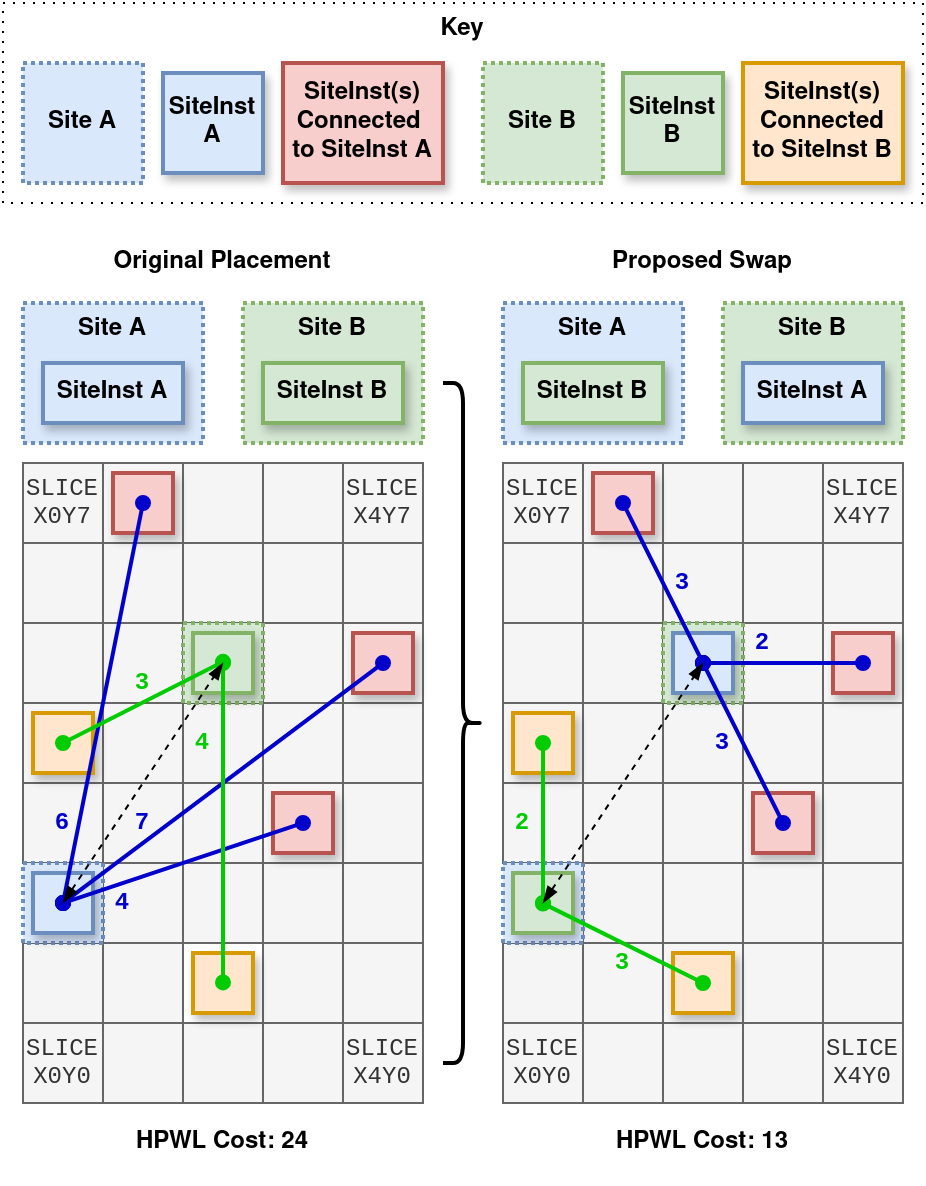
\includegraphics[width=\columnwidth]{figures/placement/swapSingleSite.png}
    \captionof{figure}{Single Site Swap Proposal}
    \label{fig:swapSingleSite}
}

\begin{lstlisting}[language=java, caption={Single Site Movement}, label={lst:sa_move_single}]
protected void moveSingleSite(List<SiteInst> sites) {
for (SiteInst si : sites) {
    SiteTypeEnum ste = si.getSiteTypeEnum();
    List<Site> homeConns = findConnectedSites(si, null);
    Site homeSite = si.getSite();
    Site awaySite = proposeSite(si, homeConns, true);
    SiteInst awaySi = occupiedSites.get(ste).get(awaySite);
    double oldCost = 0;
    double newCost = 0;
    if (awaySi != null) {
        List<Site> awayConns = findConnectedSites(awaySi, null);
        oldCost += evaluateSite(homeConns, homeSite);
        oldCost += evaluateSite(awayConns, awaySite);
        newCost += evaluateSite(homeConns, awaySite);
        newCost += evaluateSite(awayConns, homeSite);
    } else {
        oldCost += evaluateSite(homeConns, homeSite);
        newCost += evaluateSite(homeConns, awaySite);
    }
    if (evaluateMoveAcceptance(oldCost, newCost)) {
        if (awaySi != null) {
            unplaceSiteInst(si);
            unplaceSiteInst(awaySi);
            placeSiteInst(si, awaySite);
            placeSiteInst(awaySi, homeSite);
        } else {
            unplaceSiteInst(si);
            placeSiteInst(si, awaySite);
        }
    }
}
} // end randomMoveSingleSite()
\end{lstlisting}

\newcolumn
\begin{lstlisting}[language=java, caption={Cooling Schedule and Move Acceptance with Temperature}, label={lst:sa_acceptance}]
protected List<Double> coolingSchedule;
public void initCoolingSchedule(double initialTemp, double alpha, int movesLimit) {
    // geometric cooling
    double currentTemp = initialTemp;
    for (int i = 0; i < movesLimit; i++) {
        this.coolingSchedule.add(currentTemp);
        currentTemp *= alpha;
    }
}

protected boolean evaluateMoveAcceptance(double oldCost, double newCost) {
    // if the new cost is lower, accept it outright
    if (newCost < oldCost)
        return true;
    // otherwise, evaluate probability to accept higher cost
    double delta = newCost - oldCost;
    double acceptanceProbability = 
        Math.exp(-delta / this.currentTemp);
    return Math.random() < acceptanceProbability;
}
\end{lstlisting}

\begin{lstlisting}[language=Java, caption={Chain Swapping Pseudocode}, label={lst:chain_swap_pseudocode}]
protected void moveSiteChains(List<List<SiteInst>> chains) {
for (List<SiteInst> currentChain : chains) {
    int chainSize = currentChain.size();

    // Step 1: Identify home window for this chain
    Site homeAnchor = currentChain.get(0).getSite();
    List<Site> homeWindow = getSitesInWindow(homeAnchor, chainSize);

    // Step 2: Select a candidate away anchor
    Site awayAnchor = proposeAnchorSite(currentChain, homeWindow, true);

    // Step 3: Determine away window based on awayAnchor and chainSize
    List<Site> awayWindow = getSitesInWindow(awayAnchor, chainSize);

    // Step 4: Find any resident SiteInst chains in the away window
    List<List<SiteInst>> residentChainsInAway = 
        collectChainsInWindow(siteType, awayWindow);

    // Step 5: If any resident chains overlap, extend the away window to include them
    if (!residentChainsInAway.isEmpty()) {
        awayWindow = extendWindowToIncludeChains(awayWindow, residentChainsInAway);
    }

    // Step 6: Map the (possibly extended) away window back onto the original region 
    //         so that the tail of that window coincides with the tail of the current chain
    List<Site> candidateHomeWindow = mapAwayToHomeWindow(
        homeAnchor, awayWindow, chainSize);

    // Step 7: While the candidate home window still overlaps resident chains, shift upward
    int shifts = 0;
    while (windowHasOverlap(candidateHomeWindow)) {
        candidateHomeWindow = shiftWindowUp(candidateHomeWindow);
        shifts++;
        if (shifts > (homeWindow.size() - chainSize)) {
            // Reject this swap attempt and move on to the next chain
            continue;
        }
    }

    // Step 8: Compute cost of the original placement in home window
    double oldCost = evaluateWindowCost(homeWindow);

    // Step 9: Compute cost of the proposed swap placement
    double newCost = evaluateWindowCostForSwap(
        homeWindow, awayWindow, currentChain);

    // Step 10: Decide whether to accept the move based on oldCost, newCost, and temperature
    if (evaluateMoveAcceptance(oldCost, newCost, currentTemp)) {
        // Step 11: Perform an element-wise swap of SiteInsts between homeWindow and awayWindow
        swapChainsBetweenWindows(homeWindow, awayWindow);
    }
}
}
\end{lstlisting}


\newpage
\end{multicols}
{
    \centering
    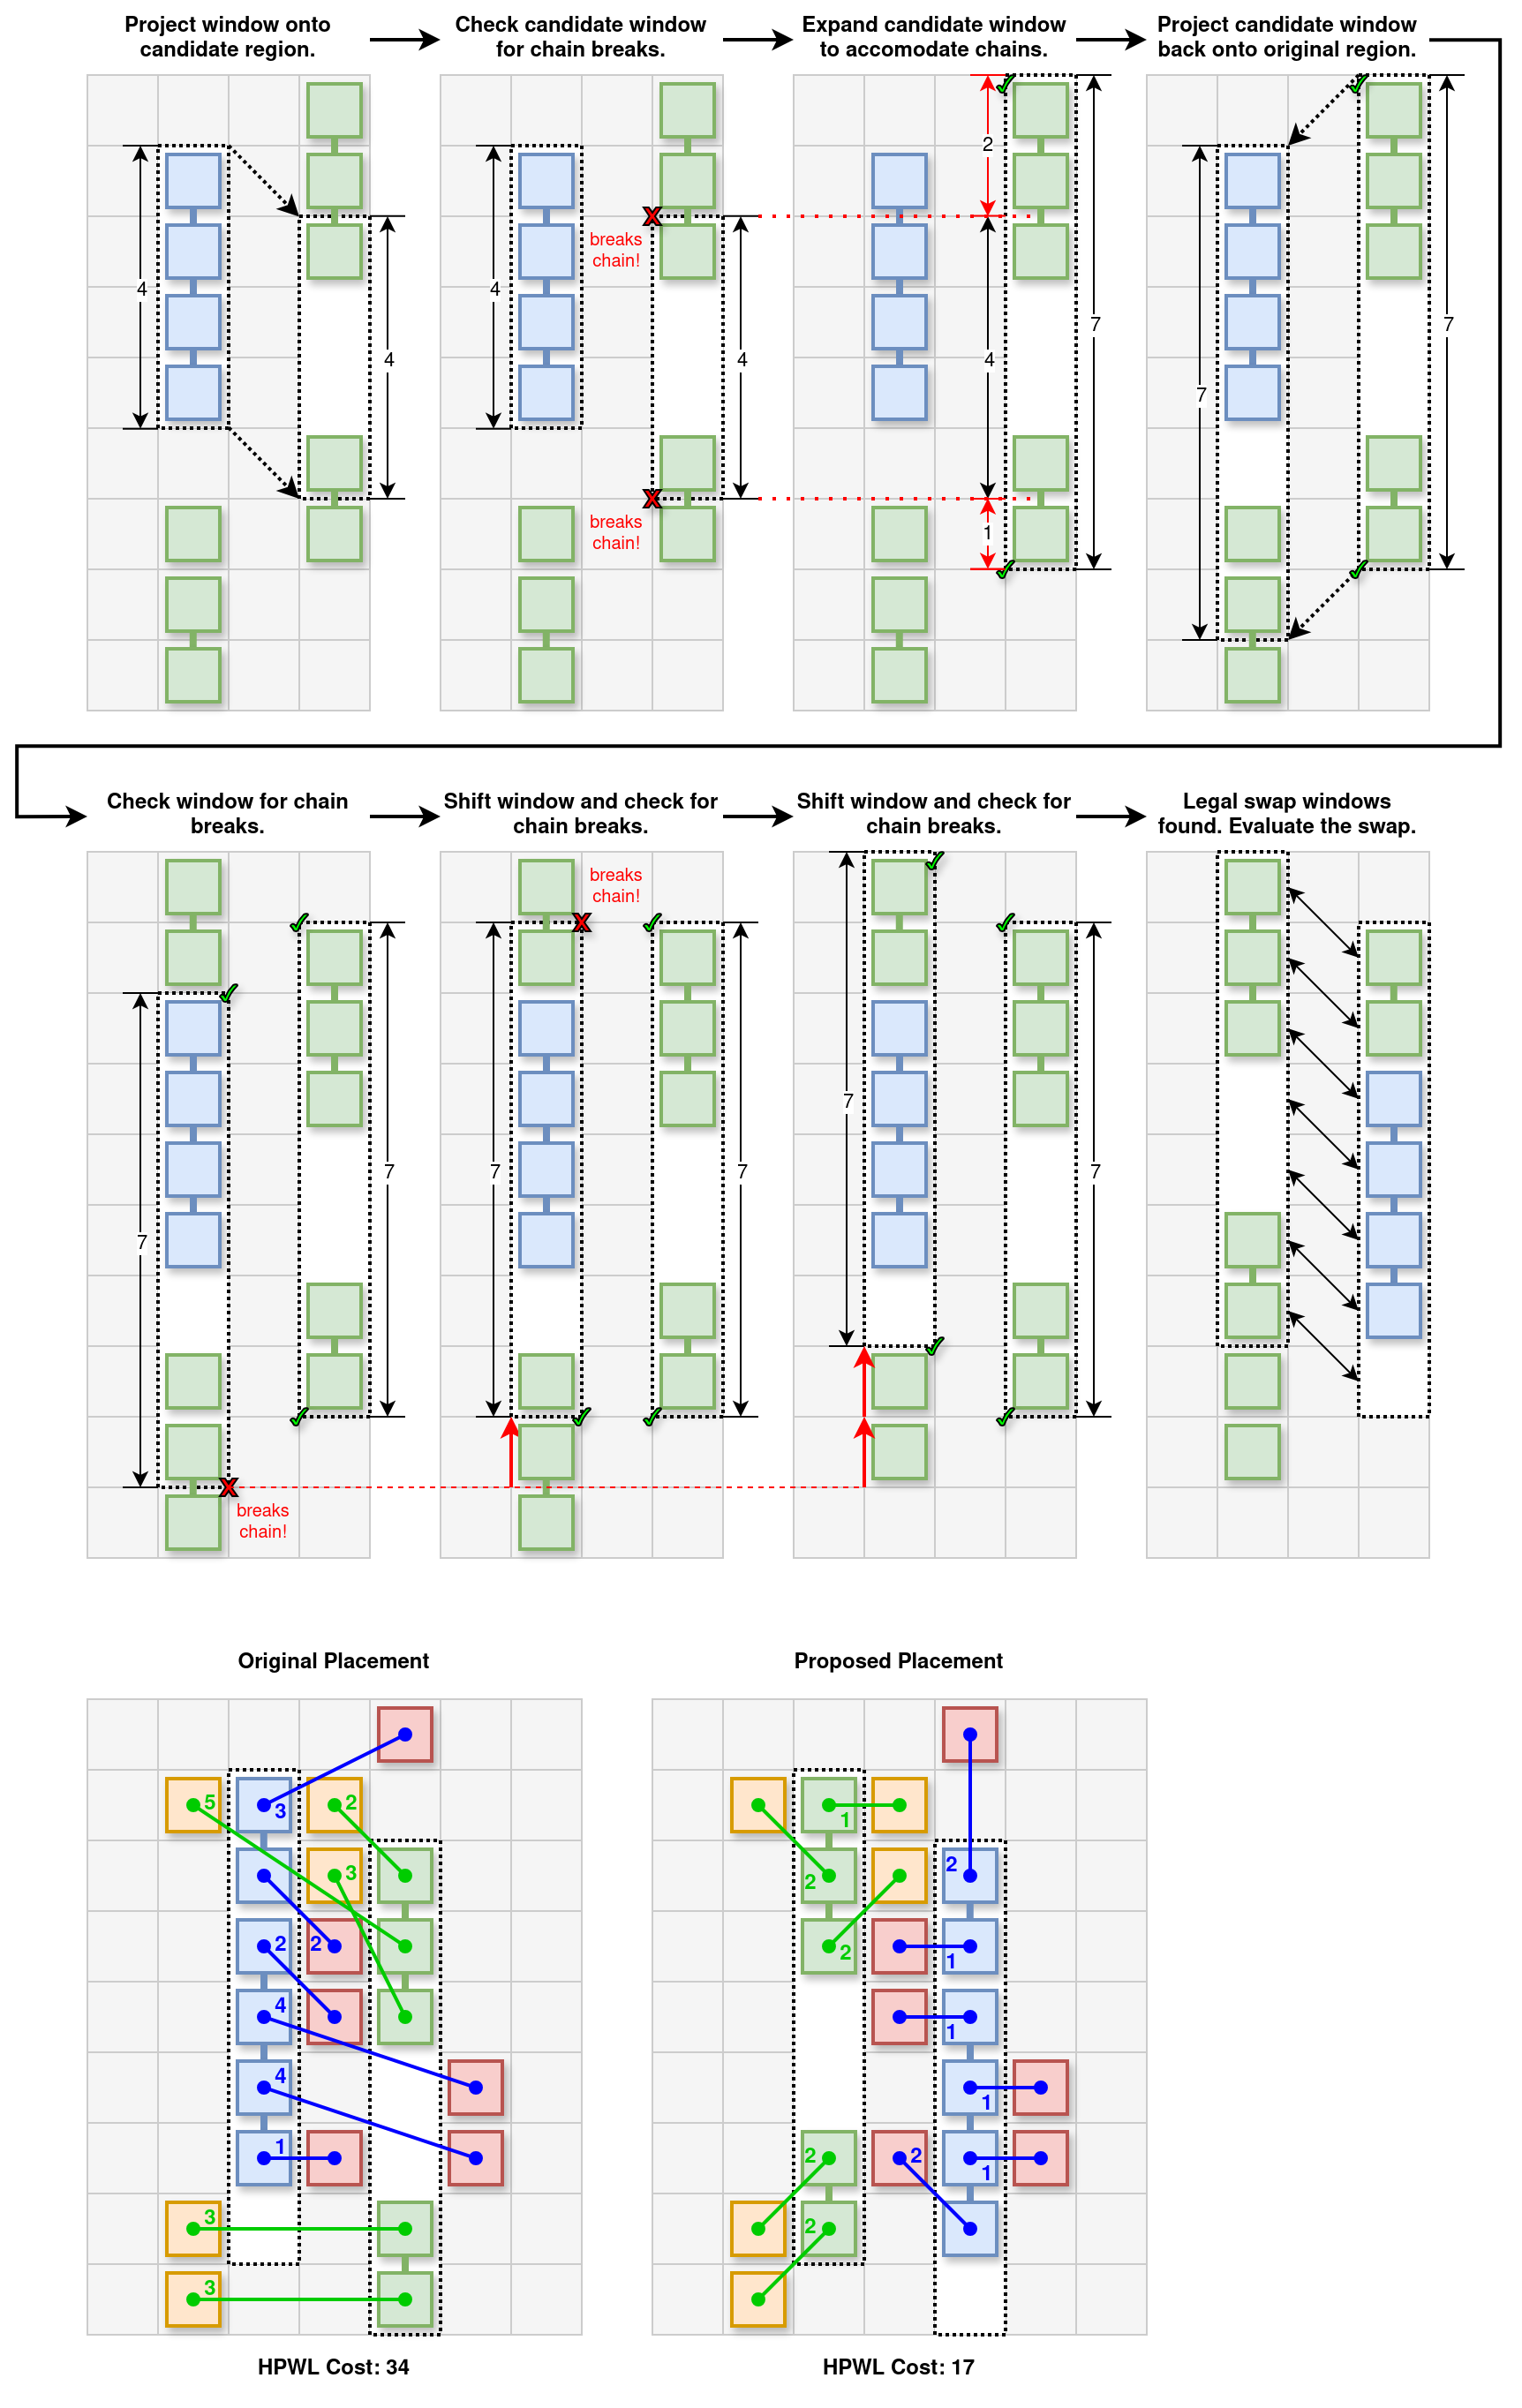
\includegraphics[width=0.9\columnwidth]{figures/placement/swapSiteChain.png}
    \captionof{figure}{Site Chain Swap Proposal}
    \label{fig:swapSiteChain}
}
\begin{multicols}{2}




